%!TEX root = ../thesis.tex
%*******************************************************************************
%****************************** Second Chapter *********************************
%*******************************************************************************

\chapter{Fabrication and Operation of Electrostatic Comb-drive Actuators in Electrolytes}

\ifpdf
    \graphicspath{{Chapter2/Figs/Raster/}{Chapter2/Figs/PDF/}{Chapter2/Figs/}}
\else
    \graphicspath{{Chapter2/Figs/Vector/}{Chapter2/Figs/}}
\fi


\section[Short title]{Chapter Overview}
In this chapter, we present examples of micro-fabricated devices that are used to study the mechanic of biological cells, and that are used in micro-fluidic systems - especially those with biological applications. Subsequently, we discuss how the electrostatic comb-drive actuator has been used to study cells, and the method by which these actuators were fabricated. We then detail the preparation of devices for experiments, and the construction of a semi-automated experimental pipeline that is used to robustly collects data on the displacement of the electrostatic comb-drive actuator in electrolytes. Finally, we enumerate the conditions under which we collect data on comb-drive displacement.

%If you have trouble viewing this document contact Krishna at: %\href{mailto:kks32@cam.ac.uk}{kks32@cam.ac.uk} or raise an issue at %\url{https://github.com/kks32/phd-thesis-template/}

%\begin{figure}[htbp!] 
%\centering    
%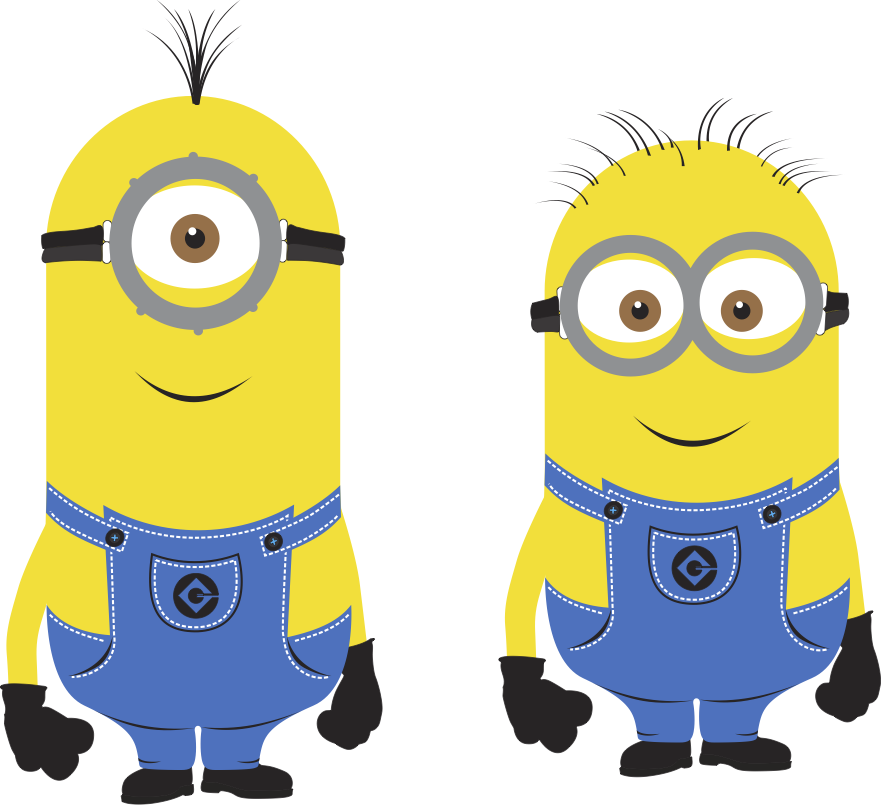
\includegraphics[width=1.0\textwidth]{minion}
%\caption[Minion]{This is just a long figure caption for the minion in %Despicable Me from Pixar}
%\label{fig:minion}
%\end{figure}


\section{Background: MEMS and Cell Characterization}
Classically, the study of biological cells was done using classic tensile devices\cite{Frisen1969,Kempson1973,Parodi1972}. These devices limited studies to collections of cells on the macroscale, and gave little insight on individual cell components. In order to overcome this limitation, biologists turned to the field of MicroelectroMechanical Systems(MEMS). Engineers in the MEMS field use a host of fabrication methods in order to construct microscale actuators and sensors that respond to mechanical, thermal, or potential signals \cite{Whitesides2001}. As a result of the size of these devices, MEMs devices are able to actuate individual components of cells at force magnitudes comparable to what they experience in their natural environments (nanoNewtons and microNewtons) \cite{Folch2000,Nianzhen2003,Vilet2003}. These properties has yielded decades of research on how forces applied to cells by surfaces with different roughness and geometric properties influence their behavior. 

The class of MEMS devices that have been developed to mechanically study cells can be generally split into two types. The first is silicon based devices that are fabricated using methods that are similar to those used to make Integrated Circuits (ICs). These devices generally have moving mechanical parts, coupled with circuitry that gives some measurement of applied force. They are constructed with dimensions that enable single cell experiments, and can also be used to facilitate the characterization of multiple individual cells simultaneously. Two major issues exist for this class of devices. The first is making the surface of these devices biocompatible, and the second is that they are not optically transparent, making it difficult to directly observe cells. However, much promising research is being done in this area. 

The second class of devices are those generated using soft-lithography, in which polymer devices are constructed by directly patterning features into their surface. These devices generally do not contain electrical components, or active mechanical parts. Instead, cells are placed on the surface of these devices, and the force the cells apply to the surface, which are patterned to provide some topography of interest, is implied from the displacement of passive mechanical structures like beams. Despite the lack of flexibility in the type of forces that can be applied to cells, soft-lithography devices have the advantage of being easy to fabricate, transparent, and easily bio-compatible. Finally, these devices allow for much smaller scales of topographic features (order 10 nanometer), making it possible to isolate which components of cells generate forces on the polymer surfaces.

%We focus on the first class of devices. A prototypical silicon device that is the dual-axis electrostatic actuator system created by Sun et al. This device was used to study single cells, and was composed of a silicon probe, attached to an electostatic comb-drive actuator. This system was used to study single cells, and was composed of a silicon probe that was attached to a comb-drive actuator on an x-y stage. The comb-drive actuator moved the probe into biological media, in order to measure the stiffness of the extracellular membrane of oocytes. \textbf{Vikram 8,68, FIGURE 2.9} 

The electrostatic comb-drive actuator in the dual-axis system is kept external to the biological media. This limitation is common among almost all electrostatic silicon devices constructed to study cell mechanics. An electrostatic actuator that is submerged in biological media, and that directly applies forces to cells is much more representative of the manner in which cells are influenced in their natural environments. Such a device would yield greater insight into the impact of forces on a variety of cells. 

In addition to micro-fabricated devices being used to directly measure the force of cells. They are also used in the context of microfluidic systems, largely with biological applications. MEMS based transdermal drug delivery (TDD) systems are one such system, figure \ref{tdd}. TDD systems are used to deliver small doses of drugs into the human body\cite{Ashraf2011}. The main componenets of these devices are an electronic control system, various electronic signal inputs, and a microfluidic device. The microfluidic device is itself composed of an actuator that pumps the fluid, valves that control the path of the fluid through the device, a reservoir, and a micro-needle. Electrostatic actuators are a popular method for controlling both the actuators, and valves \cite{Ashraf2011}.  More recently, Warnat et al. developed an enclosed MEMS microfluidic system\cite{Warnat2016}. This system was composed of MEMs structures fabricated using the Poly Multi-User MEMS process (PolyMUMPs), which were enclosed by moulds\cite{Warnat2016}. The purpose of this structure was to enable the use of MEMs devices to characterize the mechanical properties of cells in microfluidic environments\cite{Warnat2016}. Their demonstrated the feasability of thermal actuators in this context. However, operating the thermal actuators required a design that prevented these actuators from getting wet, since they caused the microfluidic liquid to boil on contact\cite{Warnat2016}. An electrostatic actuator addresses this issue. In addition allowing for a simpler overall design, an electrostatic actuator requires less power for actuation, and has faster response times.

\begin{figure}[htpb]
    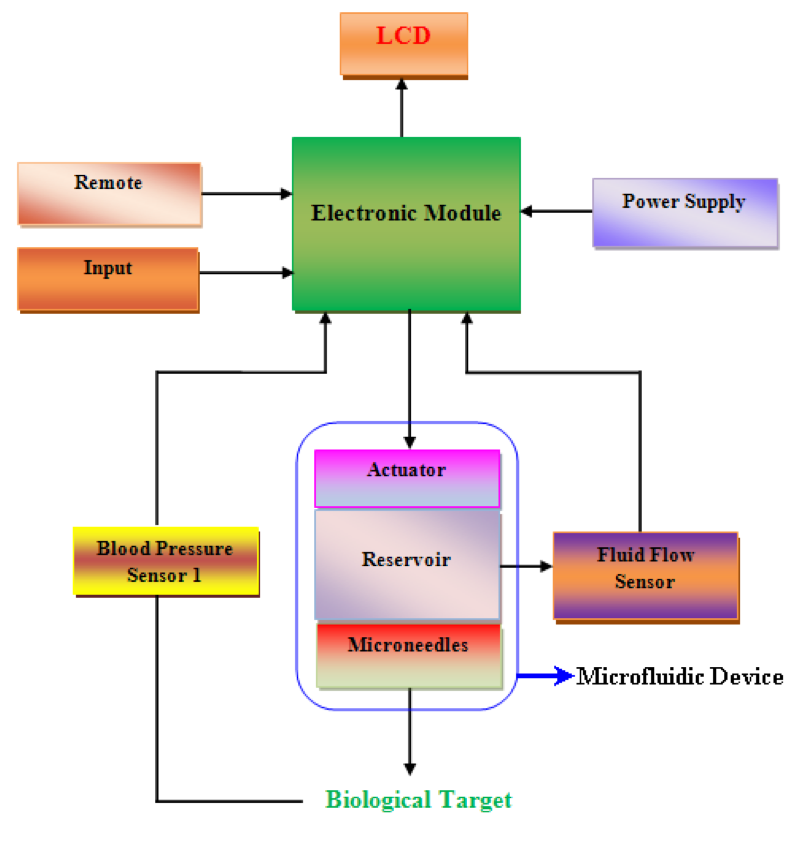
\includegraphics[width=\linewidth]{Chapter2/Figs/Raster/TDD.png}
    \caption{Diagram of transdermal drug delivery system that shows interaction of electronic system with a power suppy, and a microfluidic device corresponding to an actuator, a reservoir, and microneedles.}\label{tdd}
\end{figure}

In both the scenario in which one wishes to directly characterize the mechanical properties of cells in their natural environments, and in which one wants to construct immersed actuators for micro-fluidic systems, an electrostatic actuator that can be effectively operated in electrolytes is of critical importance.

\section{Electrostatic Comb-Drives and In Vivo Cell Characterization}
As detailed in the previous section, electrostatic comb-drive actuation in electrolytes will enable the study of cells under conditions that mimic their natural conditions. In this section, we will detail experiments that demonstrated the feasibility of using electrostatic comb-drive actuators to measure the stiffness of cells in their natural conditions. Before doing so, we review the difficulties of operating electrostatic actuators in electrolytic media, and the manner in which these difficulties were overcome. 

The behavior of the comb-drive actuator is traditionally understood by abstracting away its geometry. A common method for modeling the comb-drive is to view the overlapping components of the interdigitated fingers as a pair of parallel plates, figure \ref{finger_to_plates}. When DC voltages are applied to a comb-drive actuator in air, the potential profile between them is linear, resulting in an attractive force between the fingers. In an electrolyte, however, ions collect on the fingers and form the Stern layer and electric double layer (EDL). These layers prevent a potential drop between the fingers, thus preventing displacement in a process called ionic shielding, figure \ref{pot_profiles}. Sounart et al. discovered that this issue could be overcome by applying AC signals at frequencies faster than the time necessary for ionic shielding\cite{Sounart2005}. 

\begin{figure}[h]
    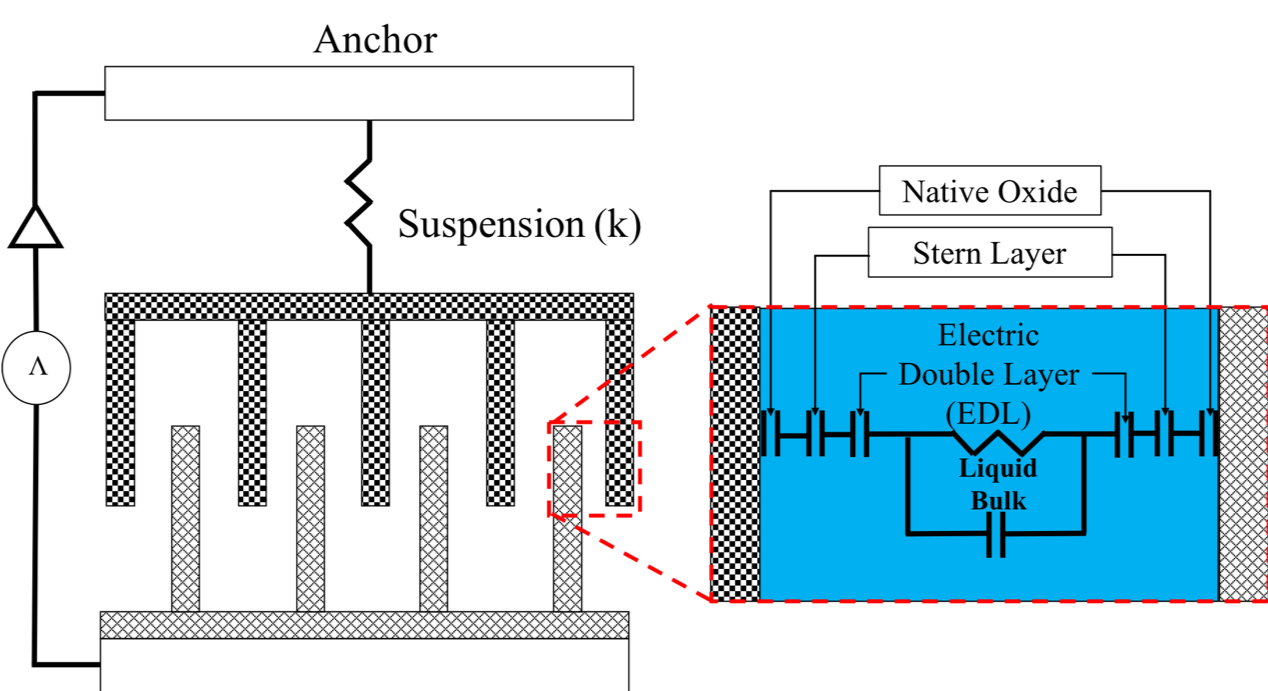
\includegraphics[width=\linewidth]{Chapter2/Figs/Raster/fingers_to_plates_electrolyte.png}
    \caption{Schematic of a comb-drive actuator, and the model of its overlapping fingers when the actuator is immersed in an electrolyte. When a voltage is applied between the inter-digitated fingers, the fingers attached to the spring move parallel to the  stationary fingers. The moving structure is grounded so that no capacitance is formed between the comb-drive and the substrate.} \label{finger_to_plates}
\end{figure}

\begin{figure}[h]
    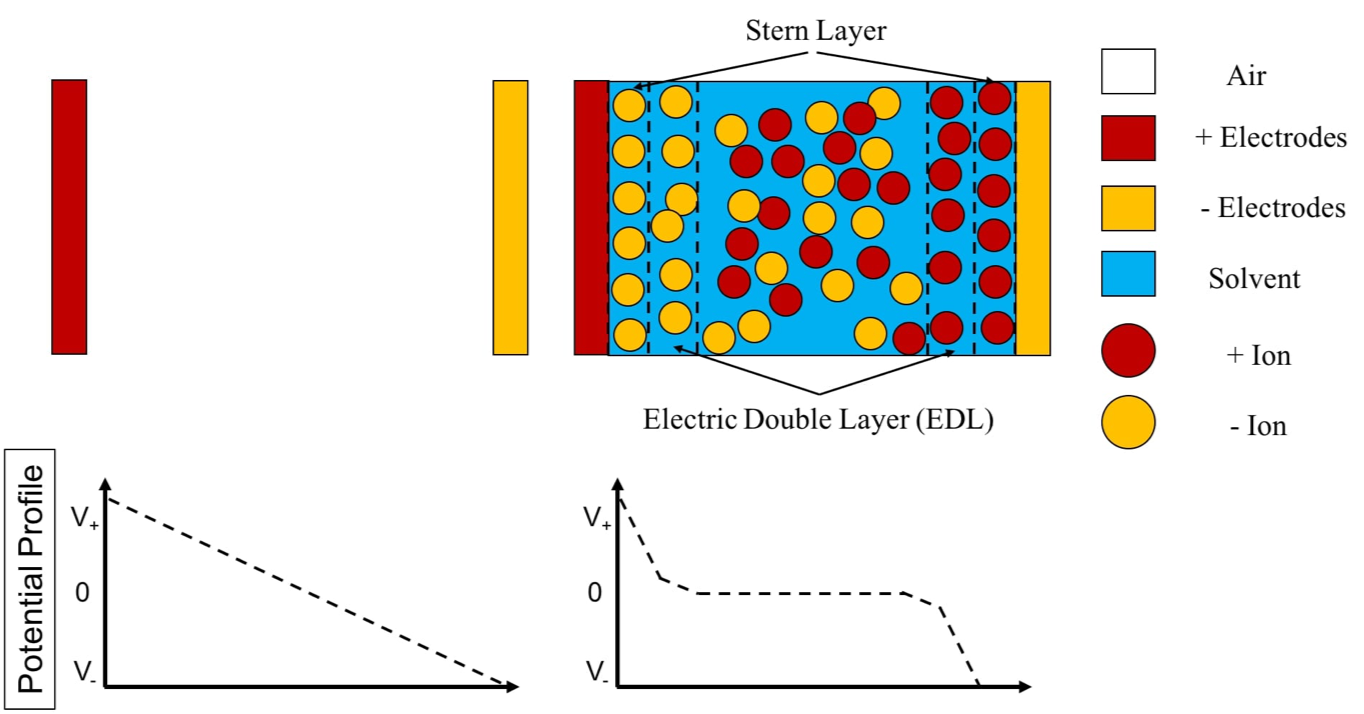
\includegraphics[width=\linewidth]{Chapter2/Figs/Raster/potprofile_air_vs_electrolyte.png}
    \caption{Pair of fingers in air (left), and electrolytes (right) under DC voltage along with their potential profiles as a function of distance between the fingers. The potential profile in air is linear, while the profile in the electrolyte is flat in the bulk, because of the voltage drop in the EDL and Stern layers.} \label{pot_profiles}
\end{figure}

\begin{figure}[htpb]
    \begin{center}
    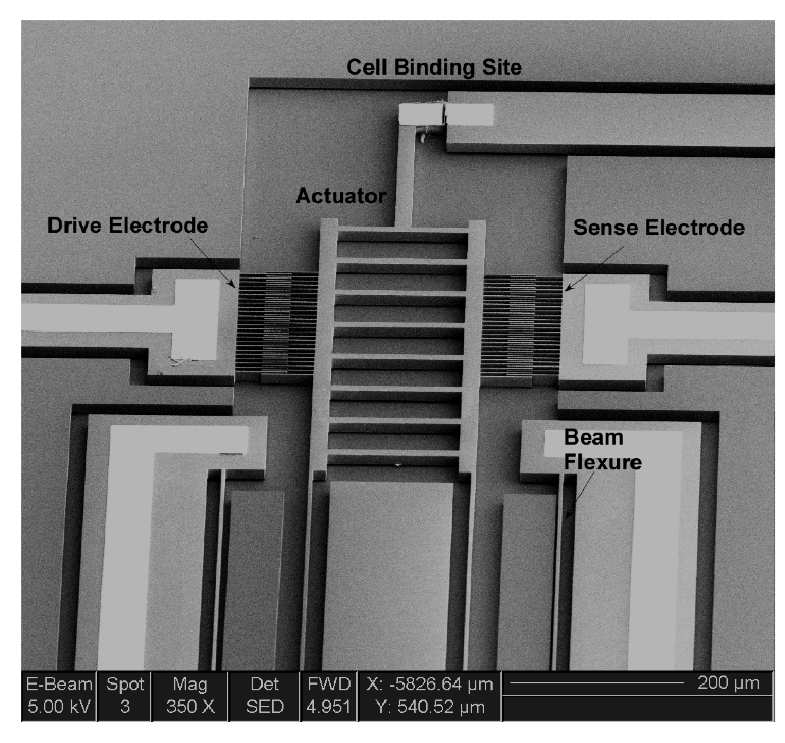
\includegraphics[width=0.6\linewidth]{Chapter2/Figs/Raster/vikramDesgn1.png}
    \caption{Image of Mukundan et al.'s first design of the comb-drive actuator to be immersed in an electrolyte.} \label{vik_design_1}
    \end{center}
\end{figure}

\begin{figure}[htpb]
    \begin{center}
    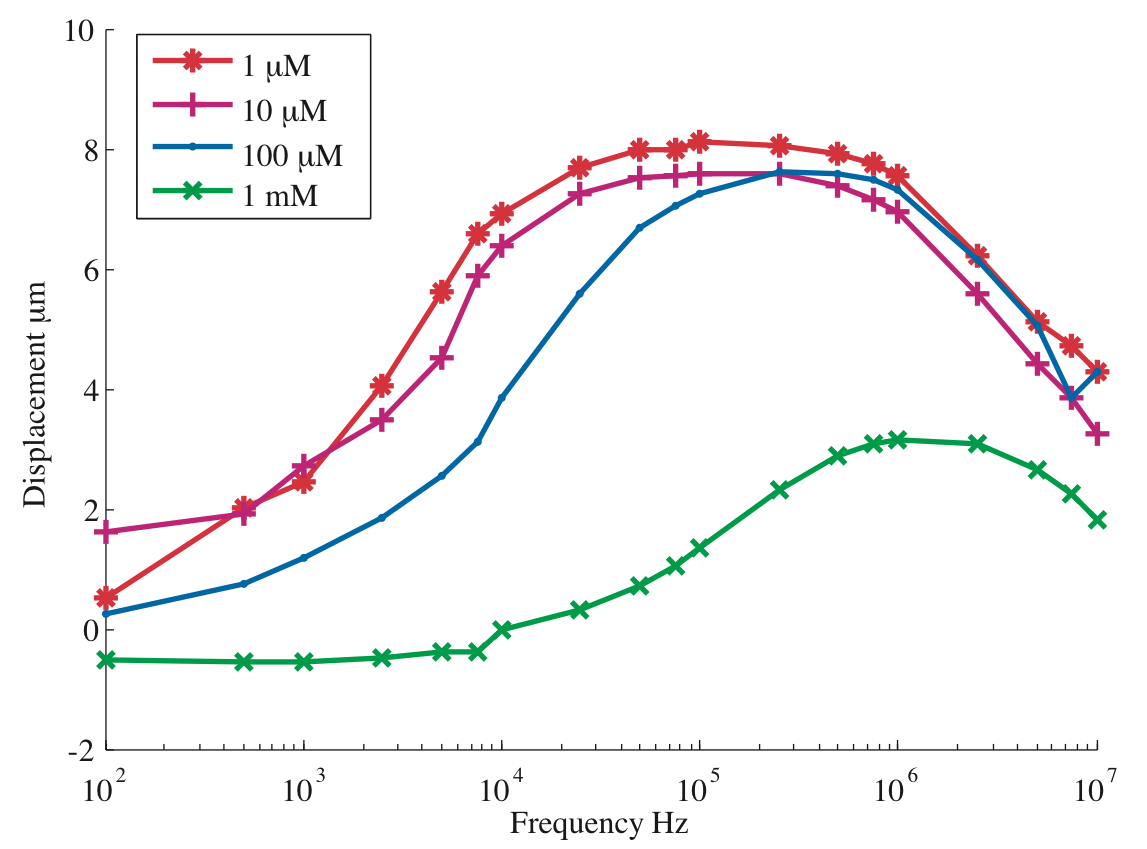
\includegraphics[width=0.6\linewidth]{Chapter2/Figs/Raster/displacementAttenuationDesgn1.png}
    \caption{Plot of displacement of the comb-drive actuator in electrolytes for Mukundan et al.'s first actuator design, as a function of frequency. The displacement decreases as frequency increases, a clear sign of parasitic impedance} \label{disp_attenuation}
    \end{center}
\end{figure}
The principle discovered by Sournat et al. were used in subsequent work by a variety of author's, in particular Mukundan et al, and Panchawagh et al \cite{Mukundan2009,MukundanandPonce2009,Panchawagh2009}. The goal of Mukundan et al.'s work was to use the comb-drive actuator in biological media, so that they could demonstrate the feasibility of using this device to actuate biological cells. The frequencies required to overcome shielding effects in biological media is minimally about one MHz. This frequency corresponds to the level at which the parasitic impedance of typical MEMs devices begins to impact their designed behavior. The originally designed device corresponds to a single flat-head tip, fabricated next to a fixed structure \cite{Mukundan2009}. This flat-head tip and fixed structure is the location to which cells were intended to bind. The flat-head tip is attached to an actuator structure. A drive comb-drive is connected to one side of the structure, and a sensor comb-drive is connected to the other, figure \ref{vik_design_1}. The end of the actuator structure furthest from the flat-head tip was attached to a folded-flexure, which facilitated its motion. When this device is operated in biological media, the distortion of the signal due to parasitic impedance results in decreasing displacement as frequencies increase above 1 MHz, figure \ref{disp_attenuation} \cite{Mukundan2009}. 

In order to overcome this, Mukundan et al. introduced what they termed a differential design, figure \ref{vik_design_2} \cite{Mukundan2009}. This structure was composed of a pair of adjacent flat-head tips, one for actuation and the other for sensing. The actuation flat-head was attached to an actuator structure with an equal number of drive comb-drives on each side. In this scenario, AC signals of opposite polarity were applied to the set of drive electrodes on each side. This resulted in approximately zero net current to the device substrate, and minimized the impact of parasitic impedance on the comb-drive actuators operation at high frequencies in biological media \cite{Mukundan2009}, figure \ref{disp_attenuation} 

\begin{figure}[htpb]
    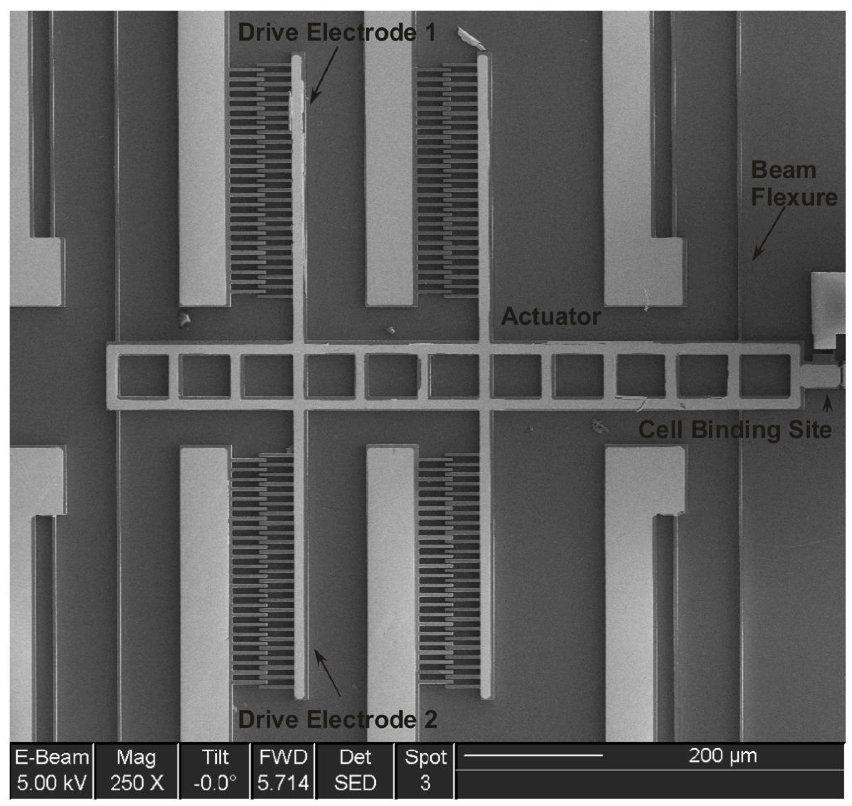
\includegraphics[width=\linewidth]{Chapter2/Figs/Raster/vikramDesgn2.png}
    \caption{Image of Mukundan et al.'s second comb-drive actuator design, which combats the issue of attenuation when actuated at high frequencies, and immersed in electrolytes} \label{vik_design_2}
\end{figure}

\begin{figure}[htpb]
    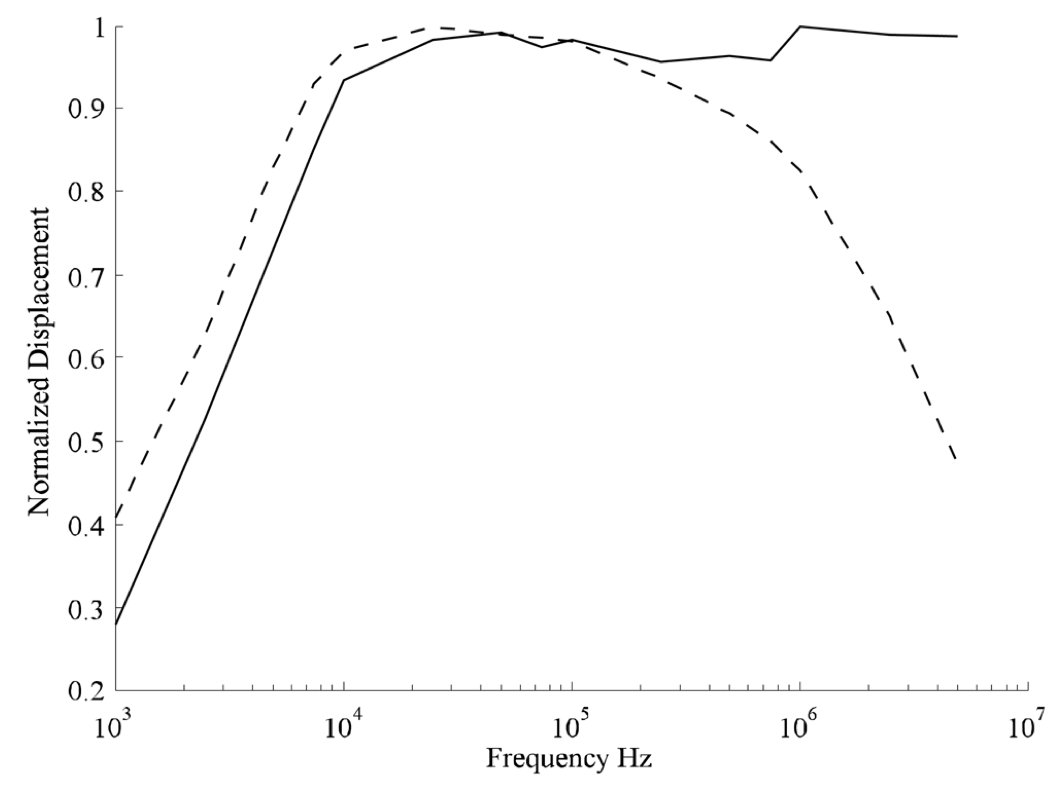
\includegraphics[width=\linewidth]{Chapter2/Figs/Raster/displacementAttenuationDesgn2.png}
    \caption{Plot of displacement of the comb-drive actuator in electrolytes for Mukundan et al.'s second actuator design, as a function of frequency. The displacement does not attenuate as severely as in the first design.} \label{vik_design_2}
\end{figure}

The final difficulty in operating comb-drive actuators in biological media is electrolysis. If AC signals of frequencies below a certain threshold are applied to the comb-drive, then electrolysis will occur at the comb-drive fingers, corroding the fingers and releasing air bubbles within the device. This threshold frequency increases as with increasing concentration. Mukundan et al. found that this could be avoided above 10 KHz for media with electrolyte concentrations at, or above, 10mM \cite{Mukundan2009}.

To the author's knowledge, the first demonstration of using a submerged electrostatic comb-drive actuator to mechanically test cells is was done by Mukundan et al. in 2009\cite{Mukundan2009}. The differential design device described earlier in this section was used to stretch Madine-Darby Canine Kidney (MDCK) cells. The flat-head tips were patterned with gold, so that the cells would adhere to them. In order to precisely place the MDCK cells on these flat-head tips, the authors used a micropipette and micromanipulator. This prevented cells from spreading through out the device, and impeding it's performance. It is important to note that the sensor flat-head tip was essentially fixed during their experiments, and that the displacement of the actuator flat-head is measured optically. The stiffness of the comb-drive device, and of the cell sample, is found by comparing the displacement and square-voltage curves of the actuating flat-head, both with and without a cell. The cell stiffness was then used to estimate the force it experienced, figure \ref{fab_steps}.

\section{Device Fabrication}
In this section, we describe how the device is fabricated, and how it is prepared for experiments. The devices were fabricated as in Mukundan et al. Specifically, they were created on silicon-on-insulator (SOI) wafers with a 15 $\micro$m device layer. The relevant features were initially patterned in the silicon through a deep reactive ion etch (DRIE) process, and E-beam evaporation was used to deposit a composite metal layer that is made of chromium (Cr 25 nm)/platinum(Pt 50 nm)/gold(Au 300 nm). Gold was used because it resists corrosion under AC voltages in electrolytes, and is bio-compatible. Finally, parylene-C was used as passivation for the electrodes. The steps in the process are shown in figure \ref{fab_steps}. 

\begin{figure}[htpb]
    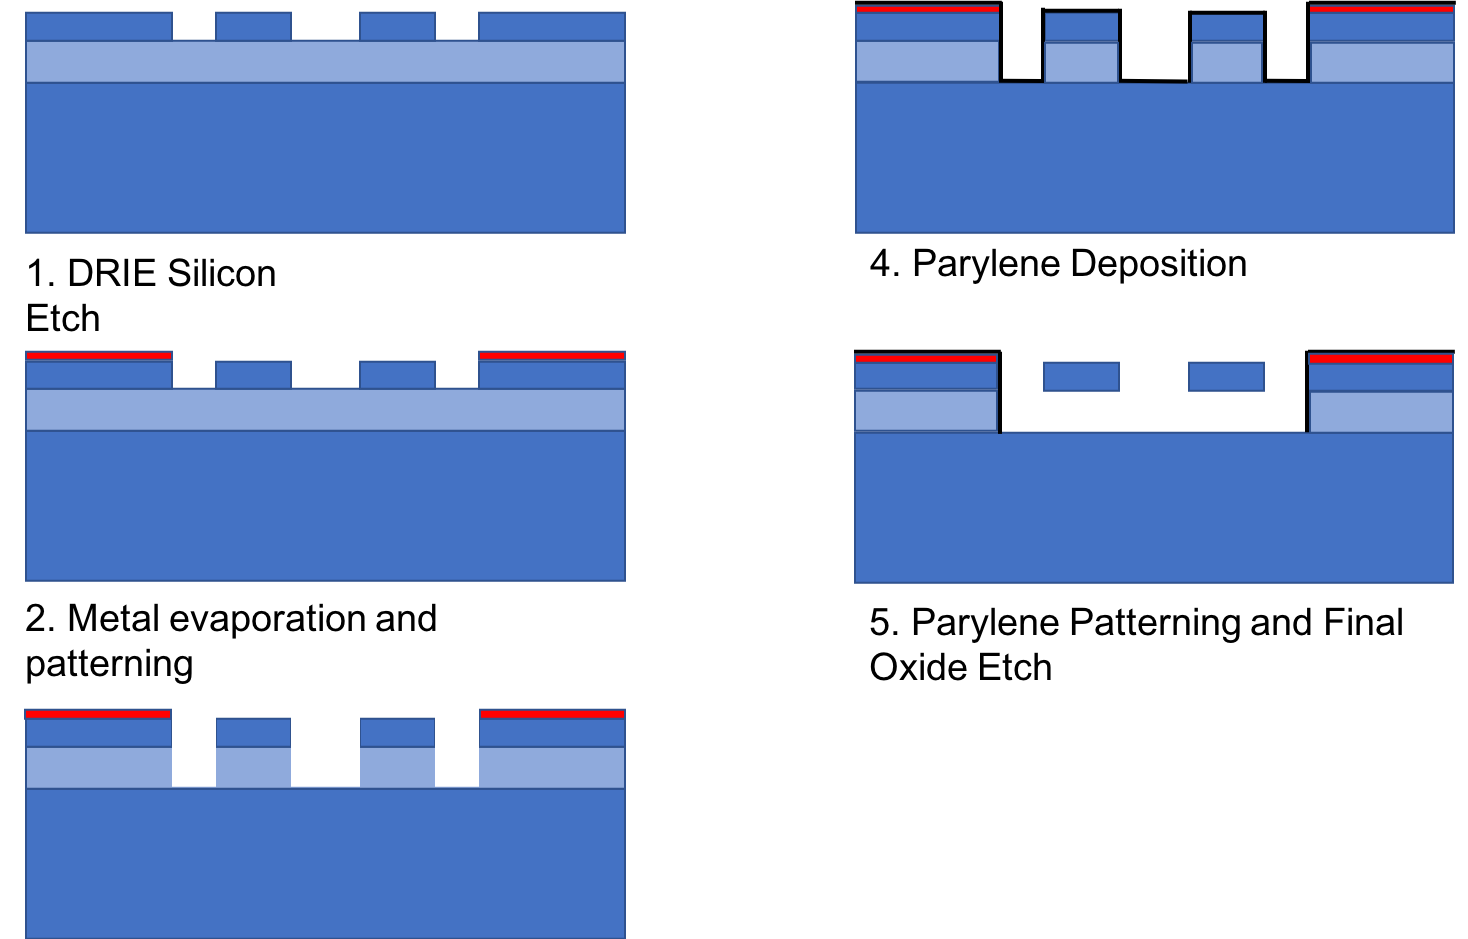
\includegraphics[width=\linewidth]{Chapter2/Figs/Raster/fabricationStepsDesgn2.png}
    \caption{Pictorial representation of sequence of fabrication steps used to create the comb-drive actuator used in this thesis, figure \ref{vik_design_2}}\label{fab_steps}
\end{figure}

\begin{algorithm}[H]
\caption{Preparing Device for Experiments}\label{euclid}
\begin{algorithmic}[1]
%\Procedure {}
\State  Micro-pipette an alcoholic solution onto the device in the DIP
\State (Optional) Immerse the entire DIP in a petri-dish of alcoholic solution, wrap it inpara-film, and allow to sit for 12-24 hours
\State $i = 0$
\While{$i \leq 8$}
    \State Micro-pipette a small amount of the alcohol out of the DIP
    \State  Micro-pipette a small amount of the aqueous solution into the DIP
    \State $i \leftarrow i+1$
\EndWhile
\State When ready to store, leave the DIP in a petri-dish of alcoholic solution, or aqueous solution and seal it with para-film.
\State \textbf{Note 1:} When replacing aqueous solution with a larger concentration of electrolytes with one with a smaller concentration, first replace the aqueous solution with alcohol, and then replace the alcohol with the new aqueous solution. The process of replacing liquids is as described in 3-5.
\State \textbf{Note 2:} Dry the device with a Critical Point Drier. If the device is allowed to dry in air, droplets will develop and damage the structure. 
%\EndProcedure
\end{algorithmic}
\end{algorithm}

\section{Preparing Device for Experiments}
The treatment of the devices post-fabrication is critical to it's successful use in experiments. The devices were mounted on ceramic dual in-line packages (DIP) using quick setting epoxy, after which the devices were allowed to sit for 12-24 hours. Gold wire-bond were then used to attach the pads on the device to the relevant pads on the DIP. Gold wire was used because it does not react with electrolytic liquids when subjected to sufficiently high frequency AC signals. The pads that correspond to the actuator structure are connected to ground, while the fixed comb-drives on either side of the actuator structure are attached to pins on the DIPs that take AC signals of opposite polarities as inputs. 

Before the device can be immersed in electrolytic liquids, it is necessary to wet it with an alcoholic solution first (at least ninety percent alcoholic), like isopropanol. If the device is immediately exposed to an electrolytic liquid, the surface tension of the aqueous solution will lead to the formation of drops that crush structures in the device, and cause irreparable deformation to the folded-flexures attached to the actuator structure. Wetting the device with alcohol first prevents the formation of drops when it is immersed in an aqueous solution. The steps of wetting are given by algorithm 1, figure \ref{wet_steps}. 

\begin{figure}[htpb]
    \begin{center}
    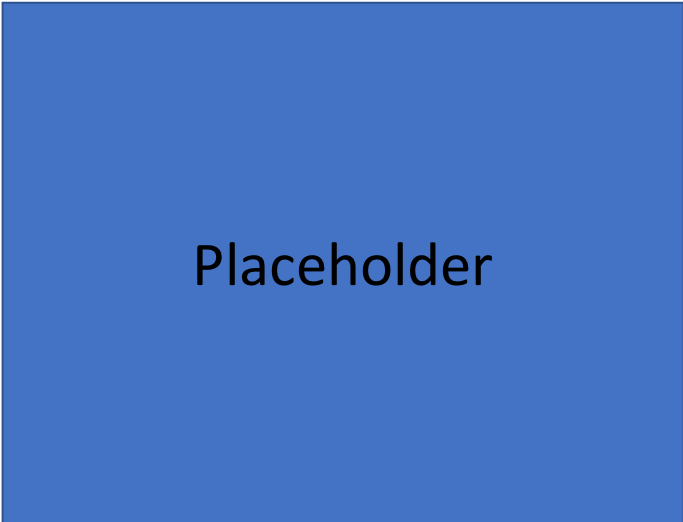
\includegraphics[width=0.3\linewidth]{Chapter2/Figs/Raster/placeholder.png}
    \caption{Placeholder for image of wetting steps}\label{wet_steps}
    \end{center}
\end{figure}


\begin{comment}
\begin{enumerate}
    \item Micro-pipette an alcoholic solution onto the device in the DIP 
    \item (Optional) Immerse the entire DIP in a petri-dish of alcoholic solution, wrap it in para-film, and allow to sit for 12-24 hours.
    \item Micro-pipette a small amount of the alcohol from the DIP
    \item Micro-pipette a small amount of the aqueous solution into the DIP
    \item Repeat steps 3 and 4 until all the liquid in the DIP is the aqueous solution
    \item When ready to store, leave the DIP in a petri-dish of alcoholic solution, or aqueous solution and seal it with para-film
    \item \textbf{Note 1:} When replacing aqueous solution with a larger concentration of electrolytes with one with a smaller concentration, first replace the aqueous solution with alcohol, and then replace the alcohol with the new aqueous solution. The process of replacing liquids is as described in 3-5.
    \item \textbf{Note 2:} Dry the device with a Critical Point Drier. If the device is allowed to dry in air, droplets will develop and damage the structure. 
\end{enumerate}
\end{comment}



\section{Experimental Pipeline}
In this section we describe the semi-automated experimental pipeline that was designed and built to collect data. We first discuss the software and hardware necessary for this pipeline. We subsequently describe how we prepare for a particular experiment, the process of running experiments, and the method by which we post-process collected data. The code associated with this is located on github, and is copied in the appendix \cite{Dibua2018DataCollect}. \textbf{Appendix}

\subsection{Software and Hardware Requirements}
The software requirements of our experimental pipeline are,

\begin{itemize}
    \item Python 2.7 or greater
    \item OpenCV (Python)
    \item Matlab
    \item GPIB Matlab
    \item Micromanager 
\end{itemize}

while the hardware requirements are

\begin{itemize}
    \item Leica Upright Microscope $\times$1
    \item TEK AFG 3102a Function Generator $\times$1
\end{itemize}

\subsection{Running an Experiment}
\subsubsection{Mounting the Device}
The process of running an experiment starts with mounting the device on the microscope, and connecting it to the function generator for the purpose of actuation. The device is submerged in an aqueous solution, following the steps described in section 2.5. This device is then placed on a chip-holder, which has been soldered to a PCB. The PCB is wired such that pins one and twenty-four are grounded, while pins three to six and nineteen to twenty-two are connected to different channels of the function generator, which applies signals that ninety degrees out of phase with each other. This PCB should already have been connected to the channels of the function generator. Figure \ref{empty_mount}, shows the chip-holder with all of the relevant connections, and figure \textbf{Image of PCB with Chip} shows DIP with the PCB.

\begin{figure}[htpb]
    \begin{center}
    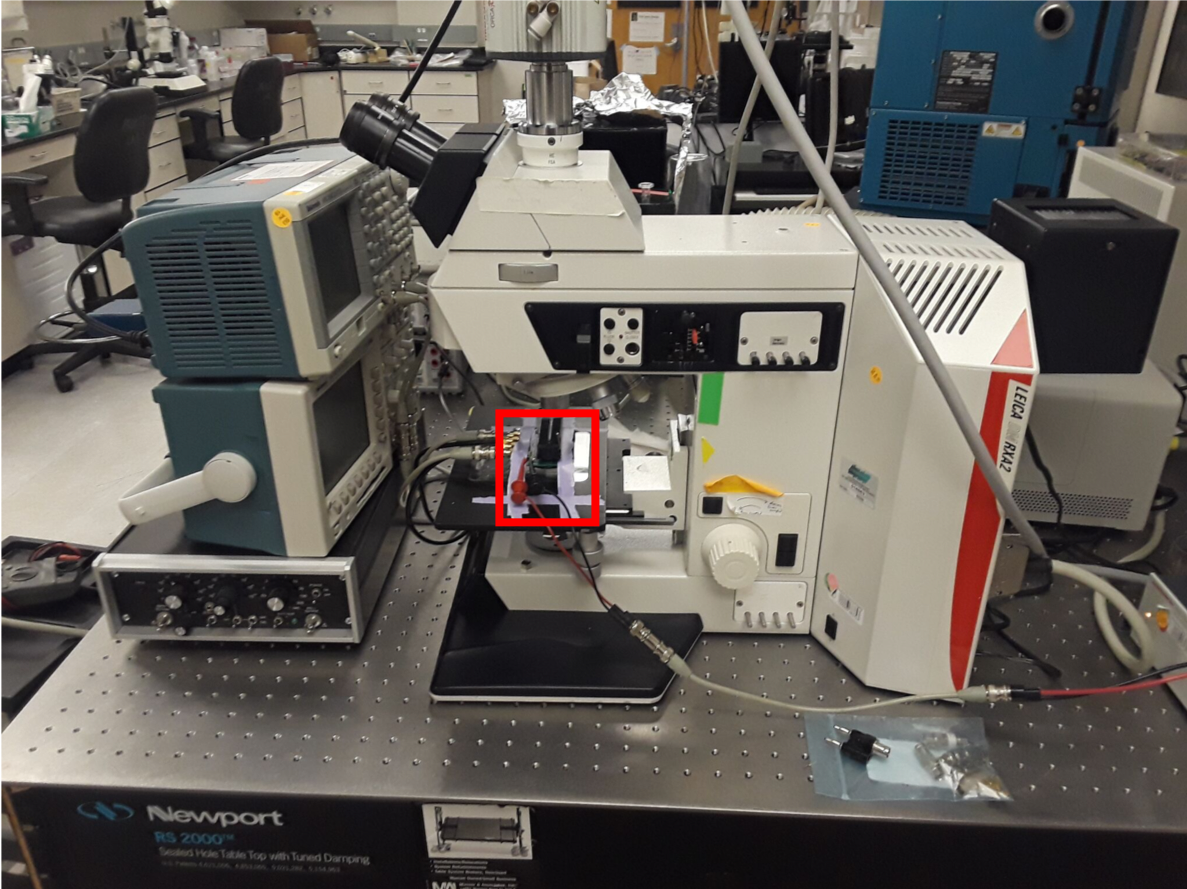
\includegraphics[width=0.8\linewidth]{Chapter2/Figs/Raster/pcb_no_dip.png}
    \caption{Image of the chip-holder on which the DIP will be mounted. The chip-holder is attached to a function generator and oscilloscope, and the tape is used to keep it flat while the microscope is moved in order to focus the image. The chip holder is bounded by a red box.}\label{empty_mount}
    \end{center}
\end{figure}

\begin{figure}[htpb]
    \begin{center}
    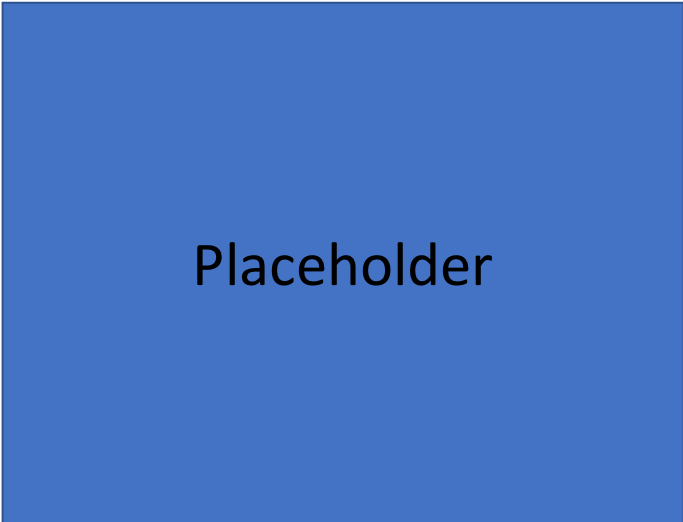
\includegraphics[width=0.5\linewidth]{Chapter2/Figs/Raster/placeholder.png}
    \caption{Placeholder for image that will show pcb mounted on a DIP}\label{pcb}
    \end{center}
\end{figure}

\begin{figure}[htpb]
    \begin{center}
    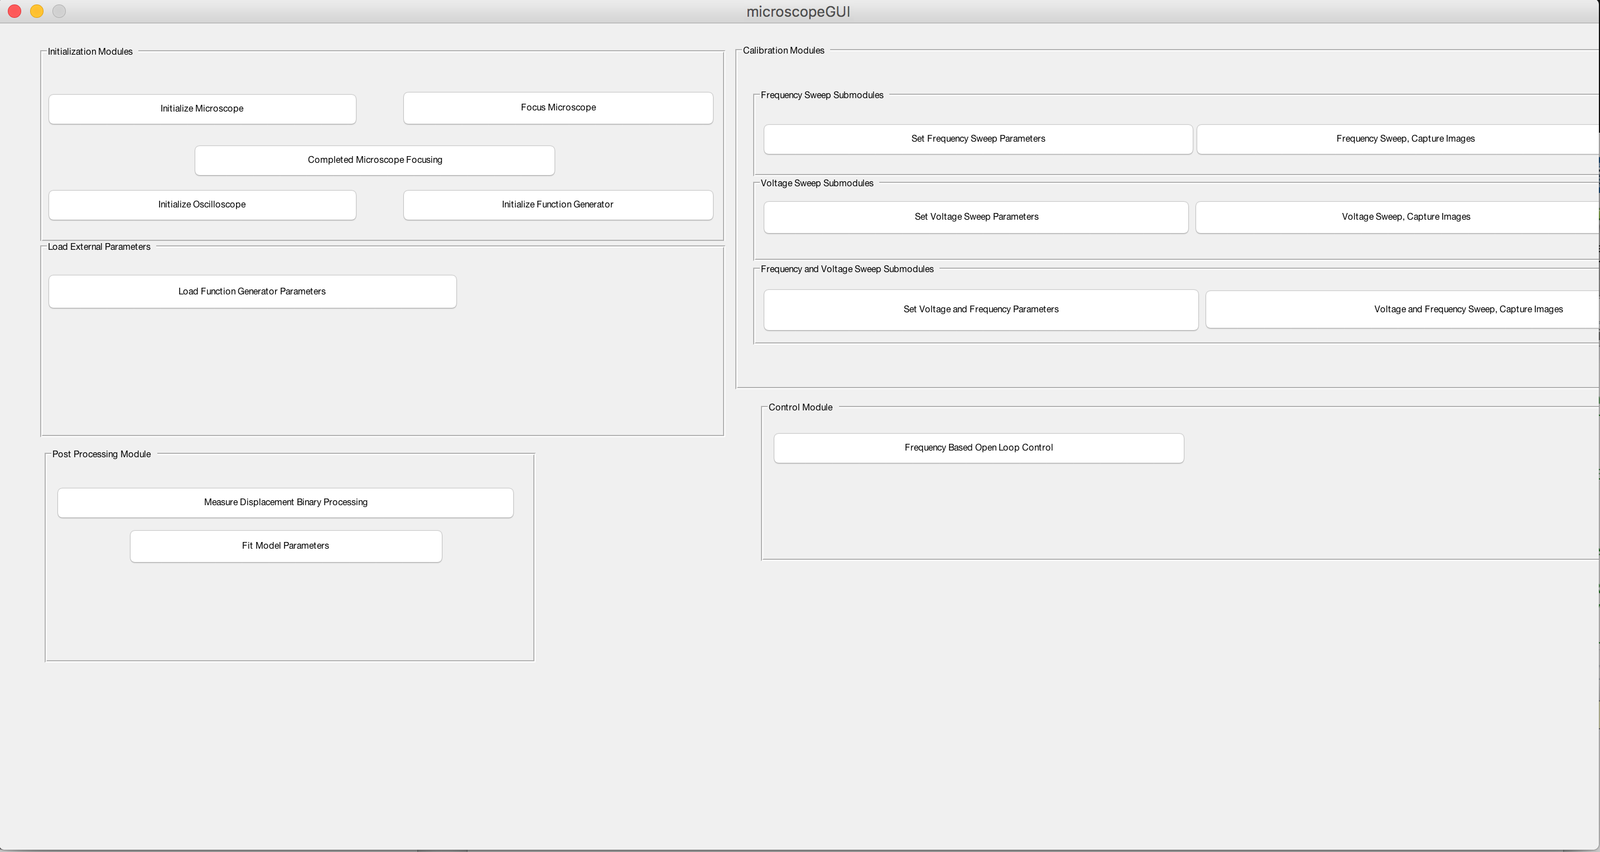
\includegraphics[width=0.9\linewidth]{Chapter2/Figs/Raster/guioptions.png}
    \caption{Options that appear when the MATLAB GUI that facilitates the semiautomatic collection of experimental data is initialized.}\label{gui_options}
    \end{center}
\end{figure}
\subsubsection{Initializing the Semi-auomated Data Collection Software}
After mounting the device, the Matlab GUI is turned on, and the microscope, function generator, and digital oscilloscope are initialized with button clicks in that order. Upon initializing the microscope, the user is asked to move the Microscope stage to a maximum and minimum height. This is will act as the bounds of the stages motion when it is moved during the process of auto-focus, and will prevent the device from crashing into the microscope lens. After this, an image of the device under the lens pops up, and the user is expected to focus the image, and click, "Complete Focus" in the GUI, after they are satisfied. 



The final aspect of initialization involves defining parameters for the experiment to be run. Clicking the Frequency sweep button will allow the user to set the maximum and minimum log of the frequency to be used in the experiment, the number of points in that range (log-spaced), the voltage of the applied signal, the number of trials to be run for these setting, and the interval of trials needed before the user is given a chance to manually focus the image, figure \ref{gui_options}. 



\subsubsection{Addressing the Challenges of Semi-automated Data Collection}
After initializing the software, the click of a button will begin the process of data collection. The channels of the function generator are set to the prescribed voltage amplitude, initialized to the proper frequency, and made 90 degrees out of phase before being turned on. Algorithm 2 outlines the manner in which the semi-automated data collection proceeds. In the algorithm, $n_{trials}$ is the number of trials chosen by the user for a particular experiment, $n_{frequency}$ the number of points selected in log space between a minimum and maximum frequency, and $n_{interval}$ is the interval of trials the user selects between which the automated data collection pauses. 


For the purpose of clarification, we will expand on some of the steps of the semi-automated data collection process. In particular, we expand upon line 16, the auto-focusing of the image, and lines 20-24, pausing data collection pending user input. During the process of running our experiments, the aqueous solution slowly evaporates. This leads to two issues. The first is that the image focus grows worse over time. The second is that the device can become dry in air, leading to damage to the comb-drive structure. 
\begin{algorithm}[H]
\caption{Semi-automated Data Collection}\label{euclid}
\begin{algorithmic}[1]
%\Procedure {}
\State Turn function generator channels off
\State Initialize function generator to $v_{init}$
\State Take and save image of device before motion
\State Initialize array of images, $I$
\State $i \leftarrow 1$
\While{$i \leq n_{trials}$}
    \If {$i=1$}
        \State Pause process pending user input
        \State Add aqueous solution to device to keep it wet
        \State Manually focus image if necessary 
        \State Turn on channels of function generator
    \EndIf
    \State $k \leftarrow 1$
    \While{$k \leq n_{frequency}$}
        \State Set function generator to the $kth$ frequency
        \State Automatically focus the image
        \State Take picture of device, and store in $I$
        \State $k \leftarrow k+1$
    \EndWhile
    \If {$rem(i,n_{interval})=0$}
        \State Pause process pending user input
        \State Add aqueous solution to device to keep it wet
        \State Manually focus image if necessary 
    \EndIf
    \State Save stored images to file
    \State $i \leftarrow i+1$
\EndWhile
%\EndProcedure
\end{algorithmic}
\end{algorithm}

\begin{algorithm}[H]
\caption{Golden-Section Search: Autofocus using GLLV}\label{euclid}
\begin{algorithmic}[1]
%\Procedure {}
\State Initialize $x_{l}*$ and $x_{u}*$
\State Initialize $x_l$ and $x_u$
\State Initialize $n_{max}$
\State Initialize $tol$
\State $k \leftarrow 1$
\While{$k<=n_{max} \text{ or } |x_l-x_u|>tol$}
    \If {$k=1$}
        \State $d = \frac{(\sqrt{5}-1)}{2}(x_u-x_l)$
        \State $x_1 = x_l + d$
        \State $x_2 = x_u - d$
    \EndIf
    \If {$x_1 < x_{u}* \text{ and } x_2 > x_{l}*$}
        \If {$f(x_1) > f(x_2)$}
            \State $x_l \leftarrow x_2$
            \State $x_2 \leftarrow x_1$
            \State $d = \frac{(\sqrt{5}-1)}{2}(x_u-x_l)$
            \State $x_1 = x_l + d$
        \Else 
            \State $x_u \leftarrow x_1$
            \State $x_1 \leftarrow x_2$
            \State $d = \frac{(\sqrt{5}-1)}{2}(x_u-x_l)$
            \State $x_2 = x_u - d$
        \EndIf
        \State $k \leftarrow k+1$
    \Else
        \State End While
    \EndIf
\EndWhile
%\EndProcedure
\end{algorithmic}
\end{algorithm}

We addressed the first issue by developing an auto-focusing algorithm. An auto-focusing algorithm has two main components. The first is defining a measure of focus that is useful for a particular application, and the second is implementing an optimization algorithm for maximizing, or minimizing, this measure. Pertuz et al. reviewed a variety of focus measures that were introduced in literature over the past two decades\cite{Pertuz2013}. Of these measures, we found that the Graylevel Local Variance (GLLV) worked well with our application. The GLLV essentially calculates the variance of the gray-levels of an image in neighborhoods of an image, and is expressed as

\begin{equation}
    \phi_{x,y} = \sum_{(i,j) \in \Omega(i,j)(x,y)} (L_{v}(i,j) - \overline{L}_v)^2,
\end{equation}

where $\phi$ is the measure, $L_{v}(i,j)$ is the variance of the gray-level in a neighborhood $w_x \times w_y$, and $\overline{L}_v$ is the mean of the gray-level in that area. This measure is maximized using the golden-section search method.

The golden-section search optimization method is constructed to find the minimum or maximum of a univariate function that is unimodal over the interval of optimization\cite{Nazareth2002}. The input to the golden-section algorithm, when optimizing the GLLV, is the height of the microscope stage. As long as the height at which the image can be focused is contained in the interval of heights being searched, the GLLV satisfies the unimodal assumption. Our implementation of the golden-section method is described in algorithm 3. In this implementation of the golden-section search, $x_l$ and $x_u$ are the minimum and maximum heights in the interval to be searched, $n_{max}$ is the maximum number of iterations of this algorithm, and $tol$ is the distance between $x_u$ and $x_l$ at which the optimization stops. Finally $x_{l}*$ and $x_{u}*$ are minimum and upper heights defined for the purposes of protecting the microscope lens. The microscope stage is should not move beyond these bounds if the optimization is properly implemented. Figure \ref{golden_section_pic} represents this algorithm pictorially.

\begin{figure}[htpb]
    \begin{center}
    
\includegraphics[width=0.6\linewidth]{Chapter2/Figs/Raster/golden_section_figure.png}
    \caption{Example of function being optimized by one step of the golden-section algorithm.}\label{golden_section_pic}
    \end{center}
\end{figure}

The second issue was addressed more simply. Rather than automating the entire experiment, we allowed the code to pause the data collection every $n$ trials, so that the user can keep the device wet.

\subsection{Post-Processing the Collected Data}
This section focuses on how the collected data is post-processed. It describes the standard method for measuring the displacement of the device pads, and the problems with robustness that this method faces. Finally, it details a new, and more robust, method for calculating the device pad displacement. We will show the impact of the different processing steps on two pads in our device when viewed using a 50x air microscope, figure \ref{orig_device}.

\begin{figure}[htpb]
    \begin{center}
    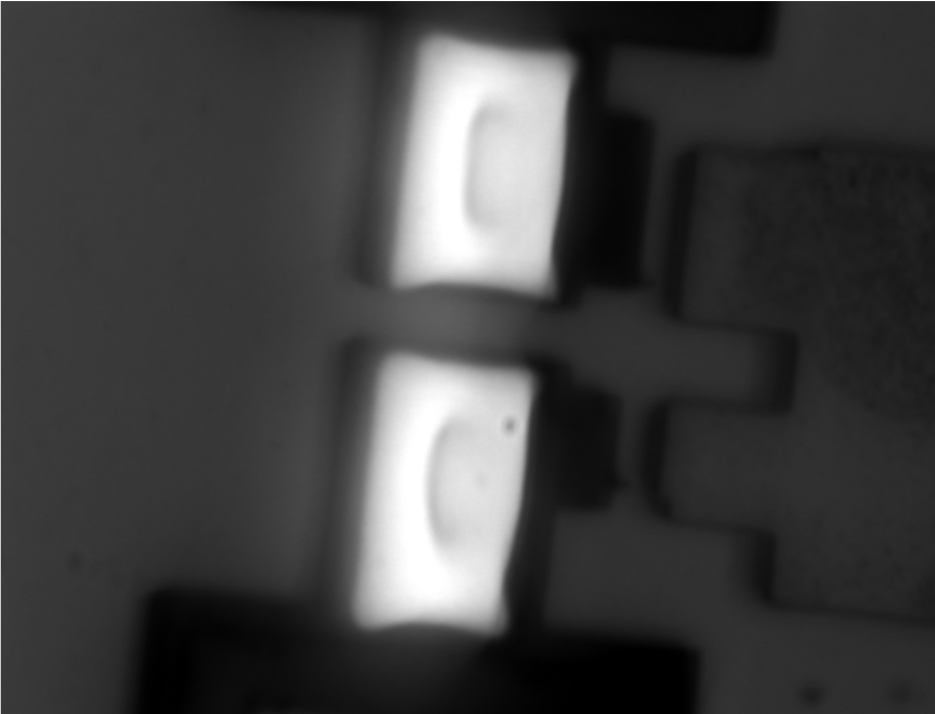
\includegraphics[width=0.6\linewidth]{Chapter2/Figs/Raster/device_processed_displace.png}
    \caption{Image of two pads of the comb-drive viewed under 50x air microscope, before any user processing.}\label{orig_device}
    \end{center}
\end{figure}

\subsubsection{Standard Method for Measuring Displacement}
The first step in measuring the displacement of the pads was transforming the image from gray-scale to binary, using a global threshold value for gray-scale intensity,$i_{th}$. This results in an image with potential holes in the contours. These holes are filled, resulting in an image with two contours corresponding to the device pads, figure \ref{binary_contour}. The device pads are then found using the area of these contours. Finally, the centroids of the contours corresponding to the pads are calculated. The change in distance between these centroids from image to image is the displacement.

This process, while promising, is not robust. In particular, this method of processing the data is sensitive to the threshold value for gray-scale intensity, $i_{th}$. Slightly different values of gray-scale intensity results in large variations of the discovered contours, and, by extension, the calculated displacement, as well as in the variance of these measurements. Figure \ref{binary_meas} shows the noisy measurements of what should be a relatively smooth pad motion, based on this processing method.
The source of this sensitivity is the change in lighting of the device that occurs over the course of an experiment. The two main sources of this change in lighting are the actuator device pad motion, and the evaporation of the aqueous solution. 

In order to credibly validate a set of models, it is critical that the data is post-processed in the most robust manner possible.

\begin{figure}
    \centering
    \begin{minipage}{0.48\textwidth}
        \centering
        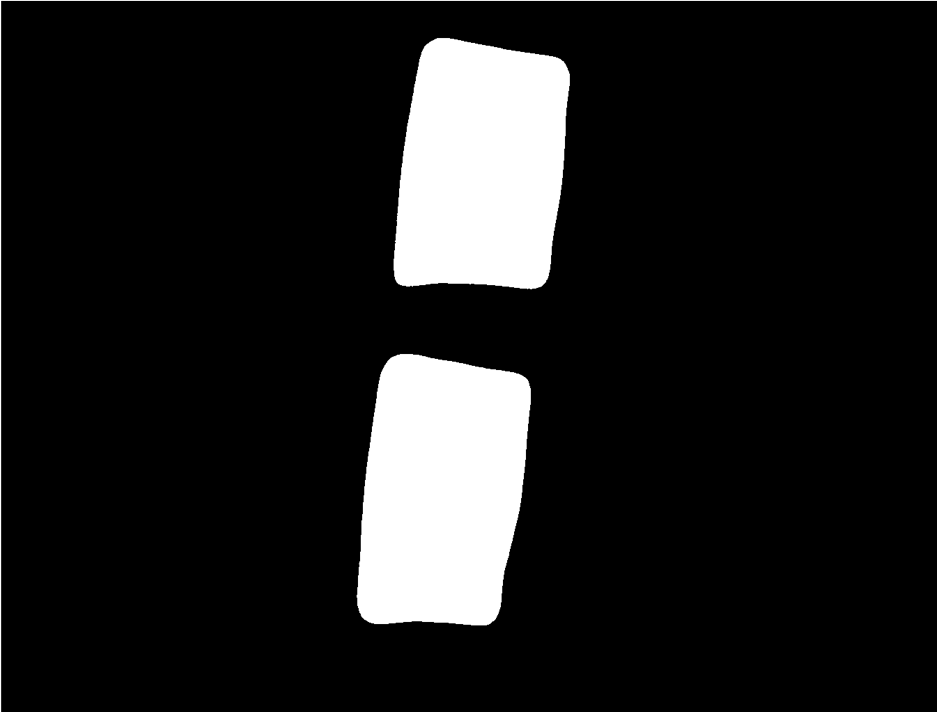
\includegraphics[width=\textwidth]{Chapter2/Figs/Raster/binary_contours.png} % first figure itself
        \caption{Binary contours found when using the standard method for measuring displacement.}\label{binary_contour}
    \end{minipage}\hfill
    \begin{minipage}{0.48\textwidth}
        \centering
        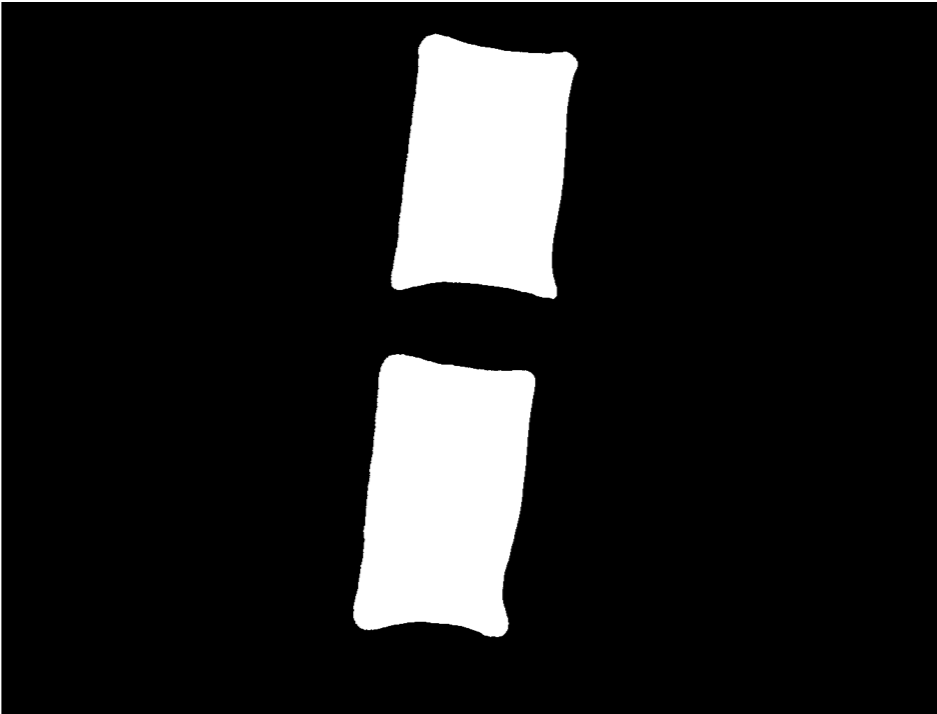
\includegraphics[width=\textwidth]{Chapter2/Figs/Raster/adaptive_contours.png} % second figure itself
        \caption{Binary contours found when using localized measure of displacement method for measuring displacement.}\label{adaptive_contour}
    \end{minipage}
\end{figure}

\subsubsection{Localized Method for Measuring Displacement}
Before discussing our alternative pipeline for measuring displacement, we briefly discuss adaptive local thresholding. Adaptive local thresholding is a method of making images binary that combats variations in illumination within, and across, images. It uses the grayscale valus of a small neighborhood, $w_x \times w_y$, around $(x,y)$ in order to determine whether or not a pixel is background or foreground. In particular,

\begin{equation}
    p(x,y) = 
        \begin{cases}
         m      & \text{if } p_0(x,y) > T(x,y) \\
         0       &   \text{otherwise} 
         \end{cases}
\end{equation}

where $p(x,y)$ is the value of pixel $(x,y)$ in the binary image, $p_0(x,y)$ is the intensity of pixel $(x,y)$ in the gray-scale image, and $T(x,y)$ is the mean gray-scale intensity of the pixels in the neighborhood of size $w_x \times w_y$ centered on $(x,y)$, sometimes subtracted from some prescribed value $c$. This particular technique is called the adaptive threshold method. It works best under the conditions in which an image contains a comparable amount of background and foreground\cite{GW2008}. When this is not the case, neighborhoods contain only foreground, or background, making this method ineffective. 

Our alternative pipeline begins by binarizing our images using local thresholding. The resulting contours are further filtered using two criteria. The first criteria are bounds on the areas of the contours, similar to the standard method for measuring displacement. The second is that the only valid contours are those that are approximately rectangles. The rest of the processing pipeline proceeds as in the standard method. The contours that results from this process closely replicate the shape of the pads in the original image and are consistent across an experiment, without needing to tune any parameters, figure \ref{adaptive_contour}, as well as yield robust measurements of displacement, figure \ref{adaptive_meas}.

\begin{figure}
    \centering
    \begin{minipage}{0.48\textwidth}
        \centering
        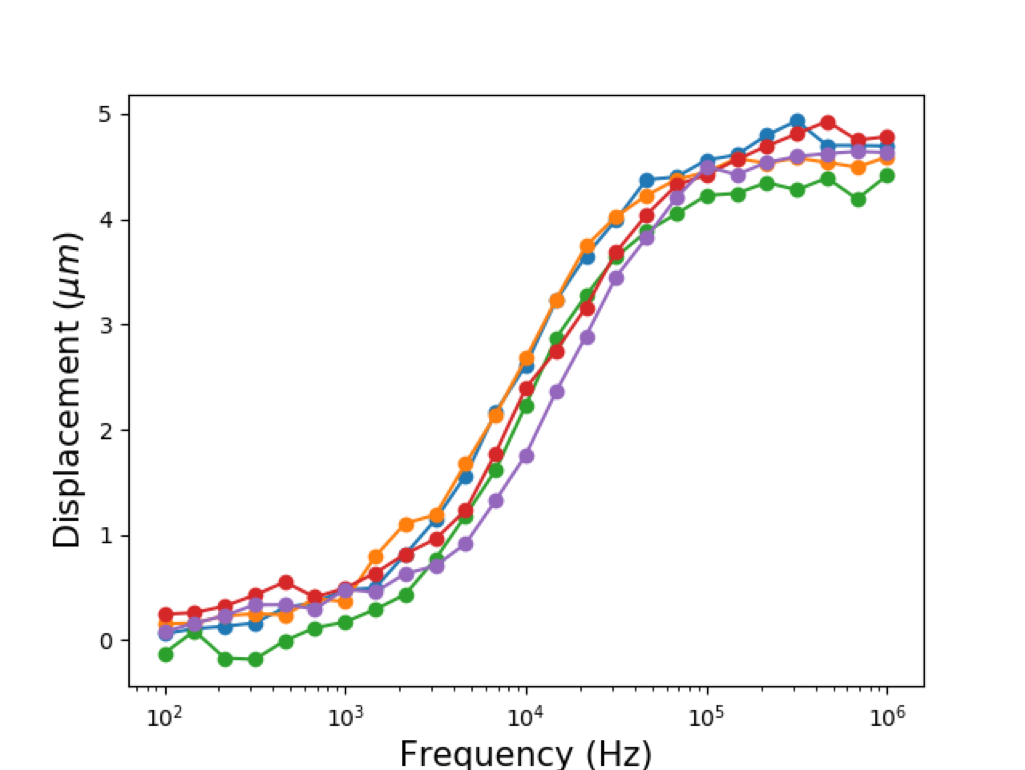
\includegraphics[width=1.1\textwidth]{Chapter2/Figs/Raster/disp_binary.png} % first figure itself
        \caption{Five trials of measured displacement of actuator pads using standard methods for measuring displacement as a function of frequency when actuated by a 4 $V_{p-p}$ signal.}\label{binary_meas}
    \end{minipage}\hfill
    \begin{minipage}{0.48\textwidth}
        \centering
        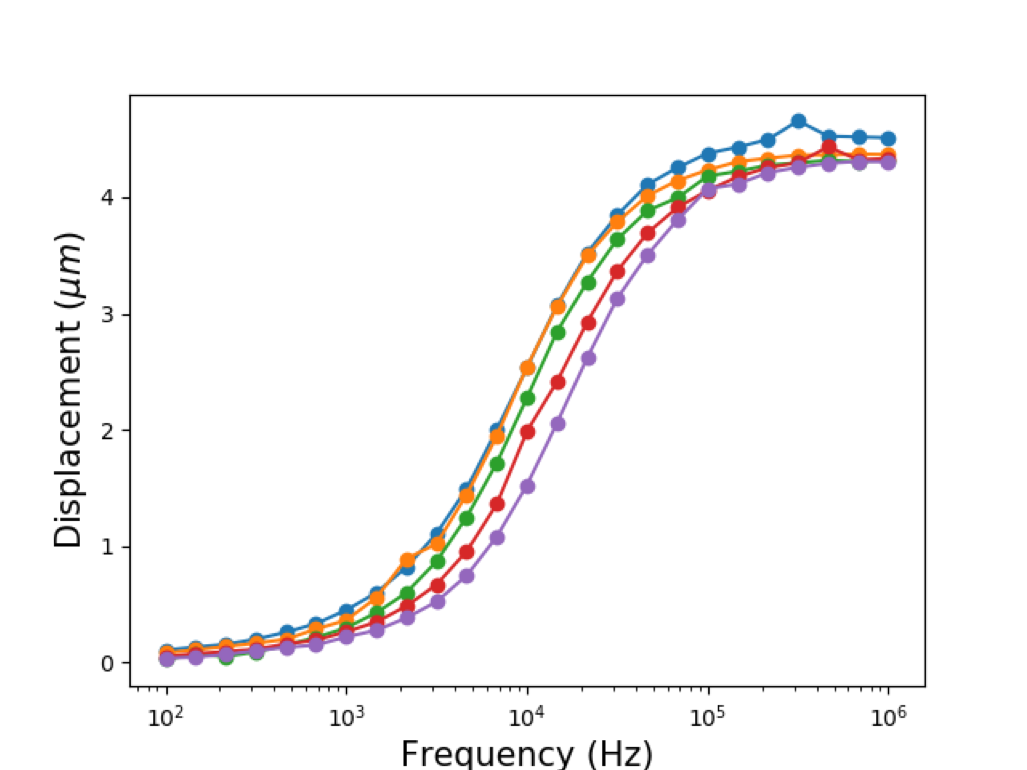
\includegraphics[width=1.1\textwidth]{Chapter2/Figs/Raster/disp_adaptive.png} % second figure itself
        \caption{Five trials of measured displacement of actuator pads using local method for measuring displacement as a function of frequency when actuated by a 4 $V_{p-p}$ signal.} \label{adaptive_meas}
    \end{minipage}
\end{figure}

\section{Experimental Conditions for Data Collection}
We have detailed the construction of a semi-automated pipeline for measuring the displacement of a comb-drive actuator in electrolytes. In this section, we detail the conditions under which we measure comb-drive displacement. We collect data at 0.1 $mM$, 0.5 $mM$, 1 $mM$, and 10 $mM$ KCl. At each concentration, we perform five trials of frequency sweeps, and, in each trial, 25 log-spaced frequencies are selected for actuation. The range of frequencies swept is from 100 $Hz$ to 1 $MHz$ at concentrations of 0.1 $mM$, 0.5 $mM$, and 1 $mM$ KCl, and between 1 $KHz$ to 10 $MHz$ for a concentration of 10 $mM$. We collect data for the described conditions for two types of comb-drive. One is a comb-drive with 200 pairs of fingers separated by a gap of 2 $\mu m$, and the second is one with 100 pairs of fingers separated by a gap of 5 $\mu m$. Unless otherwise stated, the data used for validating models will be pulled from the above described set of experiments. 
\section{Chapter Review and Further Work}
In this chapter, we gave a brief background on the use of MEMS devices to mechanically characterize cells, discussed the potential utility of electrostatic actuators in electrolytes within this context, outlined the challenges of using this electrostatic actuators in biological media (and how they were addressed), and detailed the design and implementation of an experimental pipeline that robustly calculates the displacement of the electrostatic device in an aqueous solution. 

Our experimental pipeline can be improved in two key ways. The first is in the method by which we sense displacement. Although robust, our current method of sensing displacement is relatively slow, and will limit the rate of actuation that can be applied to a cell in the context feedback control. Establishing a method for quickly sensing displacement is critical to overcoming this.  Two potential methods are fabricating markers on the device that allow the measurement of displacement without needing to process an image of the two pads in the device, or figuring out how to electrically sense displacement of an actuator in aqueous solutions.

The second flaw in our experimental pipeline is that it is only semi-automated. It requires manual interference in order to insure that the device stays wet. Creating an apparatus that automatically adds drops of the relevant aqueous solution to the device would fix this flaw, and allow for fully automated experiments. 













%\clearpage

%\tochide\section{Hidden section}
%\textbf{Lorem ipsum dolor sit amet}, \textit{consectetur adipiscing elit}. In magna nisi, aliquam id blandit id, congue ac est. Fusce porta consequat leo. Proin feugiat at felis vel consectetur. Ut tempus ipsum sit amet congue posuere. Nulla varius rutrum quam. Donec sed purus luctus, faucibus velit id, ultrices sapien. Cras diam purus, tincidunt eget tristique ut, egestas quis nulla. Curabitur vel iaculis lectus. Nunc nulla urna, ultrices et eleifend in, accumsan ut erat. In ut ante leo. Aenean a lacinia nisl, sit amet ullamcorper dolor. Maecenas blandit, tortor ut scelerisque congue, velit diam volutpat metus, sed vestibulum eros justo ut nulla. Etiam nec ipsum non enim luctus porta in in massa. Cras arcu urna, malesuada ut tellus ut, pellentesque mollis risus.Morbi vel tortor imperdiet arcu auctor mattis sit amet eu nisi. Nulla gravida urna vel nisl egestas varius. Aliquam posuere ante quis malesuada dignissim. Mauris ultrices tristique eros, a dignissim nisl iaculis nec. Praesent dapibus tincidunt mauris nec tempor. Curabitur et consequat nisi. Quisque viverra egestas risus, ut sodales enim blandit at. Mauris quis odio nulla. Cras euismod turpis magna, in facilisis diam congue non. Mauris faucibus nisl a orci dictum, et tempus mi cursus.

%Etiam elementum tristique lacus, sit amet eleifend nibh eleifend sed \footnote{My footnote goes blah blah blah! \dots}. Maecenas dapibu augue ut urna malesuada, non tempor nibh mollis. Donec sed sem sollicitudin, convallis velit aliquam, tincidunt diam. In eu venenatis lorem. Aliquam non augue porttitor tellus faucibus porta et nec ante. Proin sodales, libero vitae commodo sodales, dolor nisi cursus magna, non tincidunt ipsum nibh eget purus. Nam rutrum tincidunt arcu, tincidunt vulputate mi sagittis id. Proin et nisi nec orci tincidunt auctor et porta elit. Praesent eu dolor ac magna cursus euismod. Integer non dictum nunc.


%\begin{landscape}

%\section*{Subplots}
%I can cite Wall-E (see Fig.~\ref{fig:WallE}) and Minions in despicable me (Fig.~\ref{fig:Minnion}) or I can cite the whole figure as Fig.~\ref{fig:animations}


%\begin{figure}
%  \centering
%  \begin{subfigure}[b]{0.3\textwidth}
%    
\includegraphics[width=\textwidth]{TomandJerry}
%    \caption{Tom and Jerry}
%    \label{fig:TomJerry}   
%  \end{subfigure}             
%  \begin{subfigure}[b]{0.3\textwidth}
%    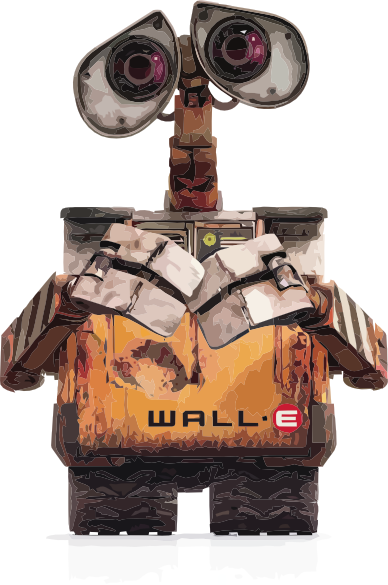
\includegraphics[width=\textwidth]{WallE}
%    \caption{Wall-E}
%    \label{fig:WallE}
%  \end{subfigure}             
%  \begin{subfigure}[b]{0.3\textwidth}
%    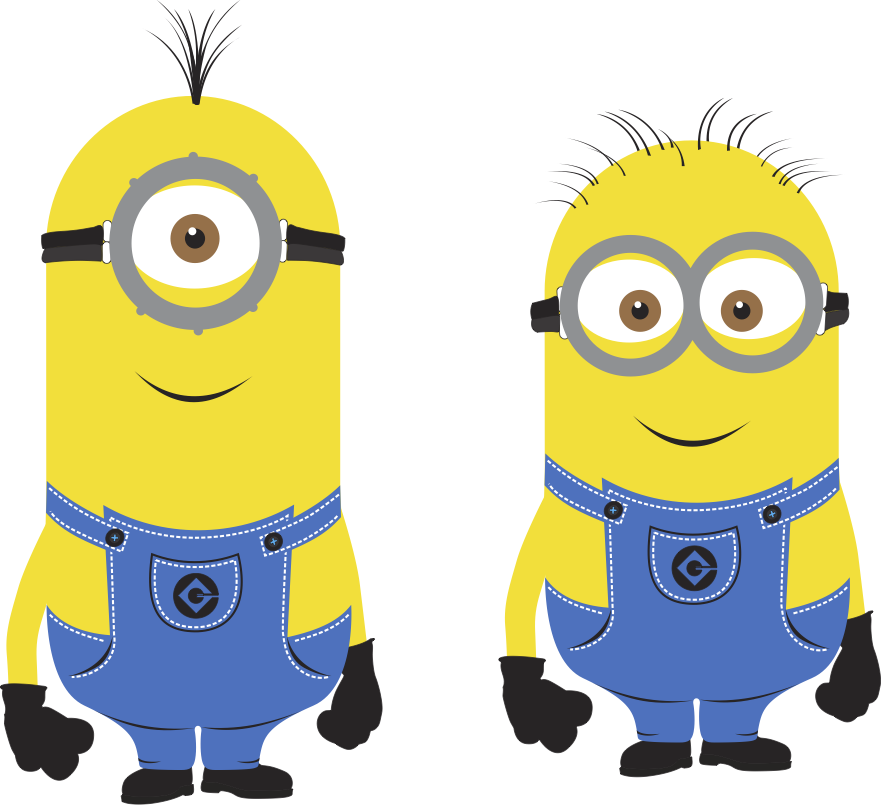
\includegraphics[width=\textwidth]{minion}
%    \caption{Minions}
%    \label{fig:Minnion}
%  \end{subfigure}
%  \caption{Best Animations}
%  \label{fig:animations}
%\end{figure}


%\end{landscape}
